\documentclass[root.tex]{subfiles}
\begin{document}

\chapter{Foundations of Mathematics}
Mathematics is the language of science. Thus, it is not designed to provide a mean of easygoing communication. Its main purpose is to test our own understanding of what we are trying to write, and to fully explore its implications. The spirit of mathematics can be summarized by the words of Ludwig Wittgenstein, who said: \emph{What we cannot speak about clearly we must pass over in silence}. Indeed, if we have a notion that we can't express in mathematical language, that is usually an indicator that some aspects have not been well understood. In this chapter, we will start with the first building block of our mathematical language: Logic. Propositional and predicate logic will allow us to write the axioms upon which all modern mathematics can be built. 

\section{Propositional logic}%{{{
The key notion of propositional logic is a proposition. 
\begin{mydef}
  A \textbf{proposition} $p$ is a variable\footnote{By this we mean a formal expression, with no extra structure assumed.} that can take the values true (T) or false (F). No other. 
\end{mydef}
This is what a proposition is, from the point of view of propositional logic. In particular, it is not the task of propositional logic to decide whether a complex statement of the form: \emph{there is extra-terrestrial life} is true or not. Propositional logic already deals with the complete proposition and it just assumes that is either true or false. Certainly, one can build new propositions from given ones by means of \textbf{logical operators}. The simplest kind of logical operators are unary operators. A unary operator takes one proposition and makes from it a new proposition. We define them in the following table:
    \begin{table}[h]
      \centering
      \begin{tabular}{c||c|c|c|c}
        $p$ & $\neg p$ & $\mathrm{id}(p)$ & $\top p$ & $\bot p$ \\
        \hline
        \rule{0pt}{12pt} F & T & F & T & F\\
                         T & F & T & T & F
      \end{tabular}\qquad
      \begin{tabular}{ll}
        $\neg$ & NOT\\
        $id$   & Identity\\
        $\top$ & Tautology\\
        $\bot$ & Contradiction
      \end{tabular}
      \caption{Unary operators}
    \end{table}

One can quickly check that, if $p$ can only be true or false, these operators cover all the possibilities to define a unary operator. The next step is to consider binary operators, i.e. operators that take two propositions and return a new one. We have 16 binary operators in total, but we draw some interesting ones in the following table:

    \begin{table}[h]
      \centering
      \begin{tabular}{c|c||c|c|c|c|c}
        $p$ & $q$ & $p\land q$ & $p\lor q$ & $p\veebar q$ & $p \Rightarrow q$ & $p \Leftrightarrow q$ \\
        \hline
          \rule{0pt}{12pt} F & F & F & F & F & T & T\\
                           F & T & F & T & T & T & F\\
                           T & F & F & T & T & F & F\\
                           T & T & T & T & F & T & T
      \end{tabular}\quad
      \begin{tabular}{ll}
        $\land$           & AND\\
        $\lor$            & OR\\
        $\veebar$         & EX-OR\\
        $\uparrow$        & NAND (not AND)\\
        $\Rightarrow$     & Implication\\
        $\Leftrightarrow$ & Equivalence
      \end{tabular}
      \caption{Some binary operators}
    \end{table}

\begin{remark}
  All higher order operators can be constructed from the single NAND operator.
\end{remark}

We point out the importance of the implication arrow, which is frequently ill-understood. The implication arrow is a binary operator that takes two propositions and constructs a new one that, in total, is true or false, as defined in the previous table.
\begin{remark}
  From the implication operator, one can conclude anything based on false assumptions, also known as ''ex falso quodlibet''.
\end{remark}
Then one may wonder why on Earth would you define the implication arrow like this. The answer is hidden in the following theorem: 
\begin{theorem}
  Let $p$, $q$ be propositions. Then $(p \Rightarrow q) \Leftrightarrow ((\neg q)\Rightarrow (\neg p))$.
\end{theorem}
\newpage
\begin{proof}
  We need only to construct the truth table and see that the two last propositions are identical:
    \begin{table}[h]
      \centering
      \begin{tabular}{c|c||c|c|c|c}
        $p$ & $q$ & $\neg p$ & $ \neg q$ & $p \Rightarrow q$ & $(\neg q) \Rightarrow (\neg p)$ \\
        \hline
          \rule{0pt}{12pt} F & F & T & T & T & T\\
                           F & T & T & F & T & T\\
                           T & F & F & T & F & F\\
                           T & T & F & F & T & T
      \end{tabular}
    \end{table}

\end{proof}

\begin{corollary}
  We can prove assertions by way of contradiction. E.g. assume that $p$ is true and we want to prove that $q$ is true. Then, what we can do instead, and is fully equivalent, is to assume that what we want to prove is not true, and then prove that the assumption is not true. Then we say we have a contradiction and $q$ must have been true.
\end{corollary}

%}}}

\section{Predicate logic}%{{{
\begin{mydef}
  A \textbf{predicate} is (informally) a proposition-valued function of some variables(s). In particular, a predicate of two variables is called a relation.
\end{mydef}

For example, $Q(x,y)$ is a proposition which value depends on the variables $x$ and $y$. Just like for propositional logic, it is not the task of predicate logic to examine how predicates are built from the variables on which they depend. Since the notions of set theory have not been yet defined, we leave it completely open, and simply consider $x$ and $y$ formal variables, with no extra conditions imposed. As with propositions, we can construct new predicates from given ones by means of the operators defined in the previous section. For example, we might have:
\begin{myex}
  $Q(x,y,z):\Leftrightarrow P(x) \land R(y,z)$
\end{myex}

More interestingly, we can construct a new proposition from a given predicate by using \emph{quantifiers}\footnote{A quantifier is a language object that specify the elements that satisfy a given predicate.}.
Let $P(x)$ be a predicate. Then, one can define the proposition
$$p:\Leftrightarrow \forall x : P(x)$$
by using the \textbf{universal quantifier} $\forall$. This means that the proposition $p$ is true $iff$, for every preposition $x$, the predicate $P(x)$ is true. $p$ is false otherwise.

Then, we can define define the \textbf{existential quantifier} $\exists$  and the \textbf{unique existential quantifier} $\exists !$ by: 
$$
\exists \, x : P(x) : \Leftrightarrow \neg (\forall \, x : \neg P(x)).
$$
$$
\exists ! \, x : P(x) :\Leftrightarrow (\exists \, x : \forall \, y : P(y) \Leftrightarrow x=y)
$$
%}}}

\section{Axiomatic System and theory of proofs}%{{{

\begin{mydef}
  An \textbf{axiom} $a$ or assumption is a proposition $p$ taken to be true, i.e. a tautology of $p$ ($a=T(p)$).
\end{mydef}

\begin{mydef}
  An \textbf{axiomatic system} is a finite sequence of axioms $a_1,a_2,\ldots,a_N$.
\end{mydef}

\begin{mydef}
  A \textbf{proof} of a proposition $p$ within an axiomatic system $a_1,a_2,\ldots,a_N$ is a finite sequence of propositions $q_1,q_2,\ldots,q_M$ such that $q_M=p$ and for any $1\leq j \leq M$ one of the following is satisfied:
\begin{enumerate}
\item[(A)] $q_j$ is a proposition from the list of axioms;
\item[(T)] $q_j$ is a tautology;
\item[(M)] $\exists \, 1\leq m,n <j : (q_m\land q_n \Rightarrow q_j)$ is true. This is called modus ponens or deduction rule.
\end{enumerate}
\end{mydef}
\begin{remark}

If $p$ can be proven within an axiomatic system $a_1,a_2,\ldots,a_N$, we write:
$$
a_1,a_2,\ldots,a_N \vdash p
$$
and we read ``$a_1,a_2,\ldots,a_N$ proves $p$''.
\end{remark}

\begin{mydef}
An axiomatic system $a_1,a_2,\ldots,a_N$ is said to be \emph{consistent} if there exists a proposition $q$ which cannot be proven from the axioms.
$$
\exists \, q : \neg (a_1,a_2,\ldots,a_N \vdash q).
$$
\end{mydef}

\begin{theorem}
  Propositional logic is consistent.
\end{theorem}

\begin{theorem}[Godel]
Any axiomatic system powerful enough to encode elementary arithmetic is either inconsistent or contains an undecidable proposition, i.e.\ a proposition that can be neither proven nor disproven within the system.
\end{theorem}
%}}}

\chapter{Axiomatic set theory}%{{{

Any space, such as the physical space, is a set "of points" equipped with further structure. But what precisely is a set? Well, one can think of a set as a collection of elements, but that raises the question of what a collection is and what elements are. So certainly we need to do better and, as a fundamental problem, if we start writing a book about mathematics whose pages are all empty yet, what could the first definition be? For a definition you need notions that you already have in order to define a new notion but, if you don't have any notion yet, how do you start? The trick is to start axiomatically, and to do so we will write axiomatic set theory. Again, this raises the question, in what language could you possibly do that? Then, we need another building block called propositional logic, which will allow us to write the axioms of set theory. 

\section{Propositional logic}%{{{
The key notion of propositional logic is a proposition. 
\begin{mydef}
  A \textbf{proposition} $p$ is a variable\footnote{By this we mean a formal expression, with no extra structure assumed.} that can take the values true (T) or false (F). No other. 
\end{mydef}
This is what a proposition is, from the point of view of propositional logic. In particular, it is not the task of propositional logic to decide whether a complex statement of the form: \emph{there is extra-terrestrial life} is true or not. Propositional logic already deals with the complete proposition and it just assumes that is either true or false. Certainly, one can build new propositions from given ones by means of \textbf{logical operators}. The simplest kind of logical operators are unary operators. A unary operator takes one proposition and makes from it a new proposition. We define them in the following table:
    \begin{table}[h]
      \centering
      \begin{tabular}{c||c|c|c|c}
        $p$ & $\neg p$ & $\mathrm{id}(p)$ & $\top p$ & $\bot p$ \\
        \hline
        \rule{0pt}{12pt} F & T & F & T & F\\
                         T & F & T & T & F
      \end{tabular}\qquad
      \begin{tabular}{ll}
        $\neg$ & NOT\\
        $id$   & Identity\\
        $\top$ & Tautology\\
        $\bot$ & Contradiction
      \end{tabular}
      \caption{Unary operators}
    \end{table}

One can quickly check that, if $p$ can only be true or false, these operators cover all the possibilities to define a unary operator. The next step is to consider binary operators, i.e. operators that take two propositions and return a new one. We have 16 binary operators in total, but we draw some interesting ones in the following table:

    \begin{table}[h]
      \centering
      \begin{tabular}{c|c||c|c|c|c|c}
        $p$ & $q$ & $p\land q$ & $p\lor q$ & $p\veebar q$ & $p \Rightarrow q$ & $p \Leftrightarrow q$ \\
        \hline
          \rule{0pt}{12pt} F & F & F & F & F & T & T\\
                           F & T & F & T & T & T & F\\
                           T & F & F & T & T & F & F\\
                           T & T & T & T & F & T & T
      \end{tabular}\quad
      \begin{tabular}{ll}
        $\land$           & AND\\
        $\lor$            & OR\\
        $\veebar$         & EX-OR\\
        $\uparrow$        & NAND (not AND)\\
        $\Rightarrow$     & Implication\\
        $\Leftrightarrow$ & Equivalence
      \end{tabular}
      \caption{Some binary operators}
    \end{table}

\begin{remark}
  All higher order operators can be constructed from the single NAND operator.
\end{remark}

We point out the importance of the implication arrow, which is frequently ill-understood. The implication arrow is a binary operator that takes two propositions and constructs a new one that, in total, is true or false, as defined in the previous table.
\begin{remark}
  From the implication operator, one can conclude anything based on false assumptions, also known as ''ex falso quodlibet''.
\end{remark}
Then one may wonder why on Earth would you define the implication arrow like this. The answer is hidden in the following theorem: 
\begin{theorem}
  Let $p$, $q$ be propositions. Then $(p \Rightarrow q) \Leftrightarrow ((\neg q)\Rightarrow (\neg p))$.
\end{theorem}
\newpage
\begin{proof}
  We need only to construct the truth table and see that the two last propositions are identical:
    \begin{table}[h]
      \centering
      \begin{tabular}{c|c||c|c|c|c}
        $p$ & $q$ & $\neg p$ & $ \neg q$ & $p \Rightarrow q$ & $(\neg q) \Rightarrow (\neg p)$ \\
        \hline
          \rule{0pt}{12pt} F & F & T & T & T & T\\
                           F & T & T & F & T & T\\
                           T & F & F & T & F & F\\
                           T & T & F & F & T & T
      \end{tabular}
    \end{table}

\end{proof}

\begin{corollary}
  We can prove assertions by way of contradiction. E.g. assume that $p$ is true and we want to prove that $q$ is true. Then, what we can do instead, and is fully equivalent, is to assume that what we want to prove is not true, and then prove that the assumption is not true. Then we say we have a contradiction and $q$ must have been true.
\end{corollary}

%}}}

\section{Predicate logic}%{{{
\begin{mydef}
  A \textbf{predicate} is (informally) a proposition-valued function of some variables(s). In particular, a predicate of two variables is called a relation.
\end{mydef}

For example, $Q(x,y)$ is a proposition which value depends on the variables $x$ and $y$. Just like for propositional logic, it is not the task of predicate logic to examine how predicates are built from the variables on which they depend. Since the notions of set theory have not been yet defined, we leave it completely open, and simply consider $x$ and $y$ formal variables, with no extra conditions imposed. As with propositions, we can construct new predicates from given ones by means of the operators defined in the previous section. For example, we might have:
\begin{myex}
  $Q(x,y,z):\Leftrightarrow P(x) \land R(y,z)$
\end{myex}

More interestingly, we can construct a new proposition from a given predicate by using \emph{quantifiers}\footnote{A quantifier is a language object that specify the elements that satisfy a given predicate.}.
Let $P(x)$ be a predicate. Then, one can define the proposition
$$p:\Leftrightarrow \forall x : P(x)$$
by using the \textbf{universal quantifier} $\forall$. This means that the proposition $p$ is true $iff$, for every preposition $x$, the predicate $P(x)$ is true. $p$ is false otherwise.

Then, we can define define the \textbf{existential quantifier} $\exists$  and the \textbf{unique existential quantifier} $\exists !$ by: 
$$
\exists \, x : P(x) : \Leftrightarrow \neg (\forall \, x : \neg P(x)).
$$
$$
\exists ! \, x : P(x) :\Leftrightarrow (\exists \, x : \forall \, y : P(y) \Leftrightarrow x=y)
$$
%}}}

\section{Axiomatic System and theory of proofs}%{{{

\begin{mydef}
  An \textbf{axiom} $a$ or assumption is a proposition $p$ taken to be true, i.e. a tautology of $p$ ($a=T(p)$).
\end{mydef}

\begin{mydef}
  An \textbf{axiomatic system} is a finite sequence of axioms $a_1,a_2,\ldots,a_N$.
\end{mydef}

\begin{mydef}
  A \textbf{proof} of a proposition $p$ within an axiomatic system $a_1,a_2,\ldots,a_N$ is a finite sequence of propositions $q_1,q_2,\ldots,q_M$ such that $q_M=p$ and for any $1\leq j \leq M$ one of the following is satisfied:
\begin{enumerate}
\item[(A)] $q_j$ is a proposition from the list of axioms;
\item[(T)] $q_j$ is a tautology;
\item[(M)] $\exists \, 1\leq m,n <j : (q_m\land q_n \Rightarrow q_j)$ is true. This is called modus ponens or deduction rule.
\end{enumerate}
\end{mydef}
\begin{remark}

If $p$ can be proven within an axiomatic system $a_1,a_2,\ldots,a_N$, we write:
$$
a_1,a_2,\ldots,a_N \vdash p
$$
and we read ``$a_1,a_2,\ldots,a_N$ proves $p$''.
\end{remark}

\begin{mydef}
An axiomatic system $a_1,a_2,\ldots,a_N$ is said to be \emph{consistent} if there exists a proposition $q$ which cannot be proven from the axioms.
$$
\exists \, q : \neg (a_1,a_2,\ldots,a_N \vdash q).
$$
\end{mydef}

\begin{theorem}
  Propositional logic is consistent.
\end{theorem}

\begin{theorem}[Godel]
Any axiomatic system powerful enough to encode elementary arithmetic is either inconsistent or contains an undecidable proposition, i.e.\ a proposition that can be neither proven nor disproven within the system.
\end{theorem}
%}}}

\section{The $\in$-relation}%{{{

Set theory is built on the postulate that there is a fundamental relation (i.e.\ a predicate of two variables) denoted by $\in$. However, there is no definition of what $\in$ is, or of what a set is. Instead, nine axioms concerning $\in$ and sets formulate the set theory upon which all modern mathematics are built. This axiomatic system is called \textbf{Zermelo-Fraenkel set theory}. As an overview, we have:

\begin{itemize}
\item 2 basic existence axioms, one about the $\in$ relation and the other about the existence of the empty set;
\item 4 construction axioms, which establish rules for building new sets from given ones.
They are the pair set axiom, the union set axiom, the replacement axiom and the power set axiom; 
\item 2 further existence/construction axioms, these are slightly more advanced and newer compared to the others;
\item 1 axiom of foundation, excluding some constructions as not being sets.
\end{itemize}
Using the $\in$-relation we can immediately define the following relations:
\begin{itemize}
  \item $x\notin y :\Leftrightarrow \neg(x\in y)$
  \item $x\subseteq y :\Leftrightarrow \forall \, a : (a\in x \Rightarrow a\in y)$
\item $x = y :\Leftrightarrow (x\subseteq y) \land (y\subseteq x)$
\item $x \subset y :\Leftrightarrow (x \subseteq y) \land \neg (x = y)$
\end{itemize}
%}}}

\section{Zermelo-Fraenkel axioms of set theory}%{{{

\subsection{Axiom on the $\in$-relation} 
The expression $x\in y$ is a proposition if, and only if, both $x$ and $y$ are sets.
$$
\forall \, x : \forall \, y : (x\in y) \veebar \neg (x\in y).
$$

\subsection{Axiom on the existence of an empty set}
There exists a set that contains no elements. $$
\exists \, y : \forall \, x : x \notin y .
$$

\begin{theorem}
This set is unique and is called the empty set $\emptyset$.
\end{theorem}

\subsection{Axiom on pair sets}
Let $x$ and $y$ be sets. Then there exists a set that contains as its elements precisely $x$ and $y$
$$
\forall \, x : \forall \, y : \exists \, m : \forall \, u : (u\in m \Leftrightarrow (u = x \lor u = y)).
$$
The set $m$ is called the \emph{pair set} of $x$ and $y$ and it is denoted by $\{x,y\}$.

\subsection{Axiom on union sets}
Let $x$ be a set. Then there exists a set whose elements are precisely the elements of the elements of $x$. 
$$
\forall \, x : \exists \, u : \forall \, y : (y \in u \Leftrightarrow \exists \, s :(y \in s\land s \in x))
$$

The set $u$ is denoted by $\bigcup x$, called union of the elements of $x$.

\subsection{Axiom of replacement}
Let $R$ be a functional relation and let $m$ be a set. Then the image of $m$ under $R$, denoted by $\text{im}_R(m)$, is again a set.

\begin{mydef}
A relation $R$ is said to be \textbf{functional} if:
$$
\forall \, x : \exists ! \, y : R(x,y) .
$$
\end{mydef}

\begin{mydef}
  Let $m$ be a set and let $R$ be a functional relation. The \textbf{image} of $m$ under $R$ consists of all those $y$ for which there is an $x\in m$ such that $R(x,y)$. 
\end{mydef}

\begin{theorem}
  Let $P(x)$ be a predicate and let $m$ be a set. Then, $\{y \in m \mid P(y)\}$ is a set. This is called \textbf{principle of restricted comprehension} and is a consequence of the axiom of replacement.
\end{theorem}

The principle of restricted comprehension is not to be confused with the ``principle'' of universal comprehension which states that $\{y \mid P(y)\} $ is a set for any predicate. This has shown to be inconsistent by Russell. Observe that the $y \in m$ condition makes it so that $\{y \in m \mid P(y)\}$ cannot have more elements than $m$ itself.


\begin{mydef}
  Let $x$ be a set. Then we define the \textbf{intersection} of $x$ by:
  $$
  \bigcap x := \{ a \in \bigcup x \mid \forall \, b \in x : a \in b \}.
  $$
\end{mydef}
If $a,b\in x$ and $\bigcap x = \emptyset$, then $a$ and $b$ are said to be \emph{disjoint}.

\begin{mydef}
  Let $u$ and $m$ be sets such that $u \subseteq m$. Then the \textbf{complement} of $u$ relative to $m$ is defined as ``$m$ without $u$'':
  $$
  m\setminus u := \{x \in m \mid x \notin u\}.
  $$
\end{mydef}

These are both sets by the principle of restricted comprehension, which is ultimately due to axiom of replacement.
\subsection{Axiom on the existence of power sets}
Let $m$ be a set. Then there exists a set, denoted by $\mathcal{P}(m)$, whose elements are precisely the subsets of $m$.

\begin{myex}
  Let $m = \{a,b\}$. Then $\mathcal{P}(m)=\{\emptyset,\{a\},\{b\},\{a,b\}\}$.
\end{myex}

%If one defines $(a,b) := \{a,\{a,b\}\}$, then the \textbf{cartesian product} $x \times y$ of two sets $x$ and $y$, which informally is the set of all ordered pairs of elements of $x$ and $y$, satisfies:
%$$
%x\times y \subseteq \mathcal{P}(\mathcal{P}(\bigcup\,\{x, y\})).
%$$
%
%Hence, the existence of $x\times y$ as a set follows from the axioms on unions, pair sets, power sets and the principle of restricted comprehension.

\subsection{Axiom of infinity}
There exists a set that contains the empty set and,  together with every other element $y$, it also contains the set $\{y\}$ as an element.
$$
\exists \, x : \emptyset \in x \land \forall \, y : (y\in x \Rightarrow \{y\} \in x).
$$

\begin{corollary}
Let us consider one such set $x$. Then $\emptyset \in x$ and hence $\{\emptyset\}\in x$. Thus, we also have $\{\{\emptyset\}\}\in x$ and so on. Therefore:
$$
x = \{\emptyset,\{\emptyset\},\{\{\emptyset\}\},\{\{\{\emptyset\}\}\},\ldots\}.
$$
We can introduce the following notation for the elements of $x$:
$$
0 :=\emptyset , \quad 1  := \{\emptyset\},\quad 2:= \{\{\emptyset\}\}, \quad 3:= \{\{\{\emptyset\}\}\} , \quad \ldots
$$
to construct the set $\mathbb{N}:=x$ and $\mathbb{R}:= \mathcal{P}(\mathbb{N})$ as known as the set of natural and real numbers respectively.
\end{corollary}

\subsection{Axiom of choice}
Let $x$ be a set whose elements are non-empty and mutually disjoint. Then there exists a set $y$ which contains exactly one element of each element of $x$.
$$
\forall \, x : P(x) \Rightarrow \exists \, y : \forall \, a \in x :\exists! \, b \in a : a \in y,
$$

where $P(x) \Leftrightarrow (\exists \,a : a \in x) \land (\forall \, a : \forall \, b : (a\in x \land b \in x) \Rightarrow \bigcap \, \{a,b\} = \emptyset )$.

\begin{remark}
The axiom of choice is independent of the other 8 axioms, which means that one could have set theory with or without the axiom of choice. However, there are important theorems that can only be proved by using the axiom of choice. 
\end{remark}

\textbf{Axiom of foundation.}\index{axiom!of foundation} \emph{Every non-empty set $x$ contains an element $y$ that has none of its elements in common with $x$. In symbols:}

$$
\forall \, x : (\exists \,a : a \in x) \Rightarrow \exists \, y \in x : \bigcap \, \{x,y\} = \emptyset .
$$

An immediate consequence of this axiom is that there is no set that contains itself as an element.\\
%}}}
%}}}

\chapter{Classification of sets}%{{{

\section{Maps}%{{{
A recurrent theme in mathematics is the classification of \emph{spaces} by means of structure-preserving \emph{maps} (homomorphisms) between them. 

\begin{mydef}
  Let $A,B$ be sets. A \textbf{map} $\phi : A \to B$ is a relation such that for each $a \in A$ there exists exactly one $b \in B$ such that $\phi(a,b)$ holds.
\end{mydef}
The standard notation for a map is:
\begin{equation}
\begin{aligned}
\phi :& A   & \to     & B\\
      & a   & \mapsto & \phi(a)
\end{aligned}
\end{equation}

The following is standard terminology for a map $\phi : A \to B$:
\begin{itemize}
  \item the set $A$ is called the \textbf{domain}\index{domain} of $\phi$;
\item the set $B$ is called the \textbf{target}\index{target} of $\phi$;
\item the set $\phi(A) \equiv \text{im}_\phi(A) := \{\phi(a) \mid a \in A\}$ is called the \textbf{image}\index{image} of $A$ under $\phi$.
\end{itemize}

\begin{mydef}
A \textbf{map} $\phi : A \to B$ is said to be:
\begin{itemize}
  \item \textbf{injective} if $\ \forall \, a_1,a_2 \in A : \phi(a_1)=\phi(a_2) \Rightarrow a_1 = a_2$;
\item \textbf{surjective} if $\text{im}_\phi(A) = B$;
\item \textbf{bijective} if it is both injective and surjective.
\end{itemize}
\end{mydef}

\begin{mydef}
  Two sets $A$ and $B$ are called \textbf{(set-theoretic) isomorphic}\index{isomorphism!of sets} if there exists a bijection $\phi : A \to B$. In this case, we write $A \cong_{set} B$.
\end{mydef}

Bijections are the ``structure-preserving'' maps for sets. Intuitively, they pair up the elements of $A$ and $B$ and a bijection between $A$ and $B$ exists only if $A$ and $B$ have the same ``size''. This is clear for finite sets, but it can also be extended to infinite sets.\\


\begin{mydef}[Classification of sets]
A set $A$ is:
\begin{itemize}
  \item \textbf{infinite}\index{set!infinite} if there exists a proper subset $B\subset A$ such that $B \cong_{set} A$. In particular, if $A$ is infinite, we further define $A$ to be:
\begin{itemize}
  \item[$*$] \textbf{countably} infinite if $A \cong_{set} \mathbb{N}$;
\item[$*$] \textbf{uncountably} infinite otherwise.
\end{itemize}
\item \textbf{finite} if it is not infinite. In this case, we have $A \cong_{set} \{1,2,\ldots,N\}$ for some $N \in \mathbb{N}$ and we say that the \textbf{cardinality} of $A$, denoted by $|A|$, is $N$.
\end{itemize}
\end{mydef}

Given two maps $\phi : A \to B$ and $\psi : B \to C$, we can construct a third map, called the \textbf{composition} of $\phi$ and $\psi$, denoted by $\psi \circ \phi$, defined by:
\begin{equation}\begin{aligned}
\psi \circ \phi : & A & \to & C\\
& a & \mapsto & \psi(\phi(a)).
\end{aligned}\end{equation}

This is often represented by drawing the following diagram
\begin{figure}[hbtp]
  \centering
\begin{tikzcd}
&B \arrow [dr,"\psi"]& \\
A  \arrow [ur,"\phi"] \arrow[rr, "\psi\circ\phi"'] & & C
\end{tikzcd}
\end{figure}

and by saying that ``the diagram commutes'' means that all paths connecting two nodes in the diagram are equivalent. 


\begin{proposition}
Composition of maps is associative.
\end{proposition}

\begin{mydef}
Let $\phi : A \to B$ be a bijection. Then the \textbf{inverse} of $\phi$, denoted $\phi^{-1}$, is defined (uniquely) by:
$$
\phi^{-1}\circ\phi = \text{id}_A
$$
$$
\phi\circ\phi^{-1} = \text{id}_B.
$$
\end{mydef}

Equivalently, we say that this diagram commutes: 
$$
\begin{tikzcd}
  A \arrow[loop left, "\text{id}_A"] \arrow[rr, bend left,"\phi"] & & B \arrow[loop right, "\text{id}_B"] \arrow[ll, bend left,"\phi^{-1}"]
\end{tikzcd}
$$

The inverse map is only defined for bijections. However, the following notion, which we will often meet in topology, is defined for any map.

\begin{mydef}
Let $\phi : A \to B$ be a map and let $V\subseteq B$. Then we define the set:
$$
\mathrm{preim}_\phi(V) := \{a \in A \mid \phi(a) \in V\}
$$
called the \textbf{pre-image} of $V$ under $\phi$.
\end{mydef}

\begin{proposition}
Let $\phi : A \to B$ be a map, let $U,V \subseteq B$ and $C=\{C_j \mid j \in J\} \subseteq \mathcal{P}(B)$. Then:
\begin{enumerate}
\item[i)] $\mathrm{preim}_\phi(\emptyset)=\emptyset$ and $\mathrm{preim}_\phi(B)=A$;
\item[ii)] $\mathrm{preim}_\phi(U\backslash V)=\mathrm{preim}_\phi(U)\backslash \mathrm{preim}_\phi(V)$;
\item[iii)] $\mathrm{preim}_\phi(\bigcup C)=\bigcup_{j \in J} \mathrm{preim}_\phi(C_j)$
 and $\mathrm{preim}_\phi(\bigcap C)=\bigcap_{j \in J} \mathrm{preim}_\phi(C_j)$.
 \end{enumerate}
\end{proposition}
%}}}

\section{Equivalence relations}%{{{

\begin{mydef}
Let $M$ be a set and let $\sim$ be a relation such that the following conditions are satisfied:
\begin{enumerate}
\item[i)] reflexivity: $\forall \, m \in M: m \sim m;$
\item[ii)] symmetry: $\forall \, m,n \in M: m \sim n \Leftrightarrow n \sim n;$
\item[iii)] transitivity: $\forall \, m,n,p \in M: (m \sim n \land n \sim p) \Rightarrow m \sim p.$
\end{enumerate}
Then $\sim$ is called an \textbf{equivalence relation}\index{equivalence relation}\index{relation!equivalence} on $M$.
\end{mydef}

\begin{myex}
Consider the following wordy examples.
\begin{enumerate}[label=\alph*)]
\item $p\sim q :\Leftrightarrow $ $p$ is of the same opinion as $q$. This relation is reflexive, symmetric and transitive. Hence, it is an equivalence relation.
\item $p\sim q :\Leftrightarrow $ $p$ is a sibling of $q$. This relation is symmetric and transitive but not reflexive and hence, it is not an equivalence relation.
\item $p\sim q :\Leftrightarrow $ $p$ is taller $q$. This relation is transitive, but neither reflexive nor symmetric and hence, it is not an equivalence relation.
\end{enumerate}
\end{myex}

\begin{mydef}
Let $\sim$ be an equivalence relation on the set $M$. Then, for any $m \in M$, we define the set:
$$
[m] := \{n \in M \mid m \sim n\}
$$
called the \textbf{equivalence class} of $m$. Note that the condition $m \sim n$ is equivalent to $n \sim m$ since $\sim$ is symmetric.
\end{mydef}

\begin{proposition}
Let $\sim$ be an equivalence relation on $M$. Then:
\begin{enumerate}
\item[i)] $a \in [m] \Rightarrow [a]=[m]$;
\item[ii)] either $[m]=[n]$ or $[m] \cap [n] = \emptyset$.
\end{enumerate}
\end{proposition}

\begin{mydef}
Let $\sim$ be an equivalence relation on $M$. Then we define the \textbf{quotient set} of $M$ by $\sim$ as:
$$
M/\!\sim\ := \{[m]\mid m \in M\}.
$$
This is indeed a set since $[m]\subseteq\mathcal{P}(M)$ and hence we can write more precisely:
$$
M/\!\sim\ := \{[m]\in\mathcal{P}(M)\mid m \in M\}.
$$
Then clearly $M/\!\sim$ is a set by the power set axiom and the principle of restricted comprehension.
\end{mydef}

\begin{remark}
Due to the axiom of choice, there exists a complete system of representatives for $\sim$, i.e.\ a set $R$ such that $R \cong_{set} M/\!\sim$.
\end{remark}

\begin{remark}
Care must be taken when defining maps whose domain is a quotient set if one uses representatives to define the map. In order for the map to be \textbf{well-defined} one needs to show that the map is independent of the choice of representatives. 
\end{remark}

%}}}

\section{\texorpdfstring{Construction of $\mathbb{N}$, $\mathbb{Z}$, $\mathbb{Q}$ and $\mathbb{R}$}{Construction of N, Z, Q and R}}%{{{

 Recall that, invoking the axiom of infinity, we defined:
 $$
 \mathbb{N} := \{0,1,2,3,\ldots\},
 $$
 where:
 $$
 0 :=\emptyset , \quad 1  := \{\emptyset\},\quad 2:= \{\{\emptyset\}\}, \quad 3 := \{\{\{\emptyset\}\}\} , \quad \ldots
 $$
 We would now like to define an addition operation on $\mathbb{N}$ by using the axioms of set theory. We will need some preliminary definitions.

\begin{mydef}
  The \emph{successor map} $S$ on $\mathbb{N}$ is defined by:
  \begin{align*}
   S :\ & \mathbb{N}  \rightarrow \mathbb{N}\\
       & n \mapsto \{n\}
  \end{align*}
\end{mydef}

\begin{mydef}
  The \emph{predecessor map} $S$ on $\mathbb{N}^* := \mathbb{N}\setminus \emptyset$ is defined by:
  \begin{align*}
   S :\ & \mathbb{N}  \rightarrow \mathbb{N}\\
       & n \mapsto m \quad \text{such that } \{m\} = n
  \end{align*}
\end{mydef}

\begin{mydef}
Let $n \in \mathbb{N}$. The \emph{$n$-th power} of $S$, denoted $S^n$, is defined recursively by:
\begin{align*}
  &S^n := S \circ S^{P(n)} \qquad \text{if } n \in \mathbb{N}^*\\ 
  &S^0 := id_\mathbb{N}
\end{align*}
We are now ready to define addition.
\end{mydef}

\begin{mydef}
The \emph{addition} operation on $\mathbb{N}$ is the map:
\begin{align*}
   + :\ & \mathbb{N} \times \mathbb{N}  \rightarrow  \mathbb{N}\\
   & (m,n)  \mapsto  m +n:= S^n(m).
\end{align*}
\end{mydef}

\begin{mydef}
Let $\sim$ be the equivalence relation on $\mathbb{N}\times \mathbb{N}$ defined by:
$$
 (m,n) \sim (p,q) :\Leftrightarrow m+q = p+n.
$$
\end{mydef}

\begin{mydef}
 We define the set of \emph{integers} by:
$$
\mathbb{Z}\index{$\mathbb{Z}$}:=(\mathbb{N}\times\mathbb{N})/\!\sim.
$$
\end{mydef}

The intuition behind this definition is that the pair $(m,n)$ stands for ``$m-n$''. In other words, we represent each integer by a pair of natural numbers whose (yet to be defined) difference is precisely that integer. There are, of course, many ways to represent the same integer with a pair of natural numbers in this way. For instance, the integer $-1$ could be represented by $(1,2)$, $(2,3)$, $(112,113)$, \ldots

\begin{remark}
 In a first introduction to set theory it is not unlikely to find the claim that the natural numbers are part of the integers, i.e.\ $\mathbb{N} \subseteq \mathbb{Z}$. However, according to our definition, this is obviously nonsense since $\mathbb{N}$ and $\mathbb{Z}:=(\mathbb{N}\times\mathbb{N})/\!\sim$ contain entirely different elements. What is true is that $\mathbb{N}$ can be \emph{embedded} into $\mathbb{Z}$, i.e.\ there exists an \emph{inclusion map} $\iota$, given by:
\begin{align*}
  \iota :\ & \mathbb{N} \hookrightarrow  \mathbb{Z}\\
 & n  \mapsto  [(n,0)]
\end{align*}
and it is in this sense that $\mathbb{N}$ is included in $\mathbb{Z}$.
\end{remark}

\begin{mydef}
Let $n := [(n,0)] \in \mathbb{Z}$. Then we define the \emph{inverse} of $n$ to be $-n:=[(0,n)]$. 
\end{mydef}

We would now like to inherit the $+$ operation from $\mathbb{N}$.

\begin{mydef}
We define the \emph{addition of integers} $+_\mathbb{Z}:\ \mathbb{Z}\times\mathbb{Z}\to\mathbb{Z}$ by:
$$
[(m,n)] +_\mathbb{Z} [(p,q)] := [(m+p,n+q)].
$$
\end{mydef}


\begin{mydef}
In a similar fashion, we define the set of \emph{rational numbers} by:
$$
\mathbb{Q}\index{$mathbb{Q}$} := (\mathbb{Z}\times\mathbb{Z}^*)/\!\sim,
$$
where $\mathbb{Z}^*:=\mathbb{Z}\setminus\{0\}$ and $\sim$ is a relation on $\mathbb{Z}\times\mathbb{Z}^*$ given by:
$$
(p,q)\sim(r,s) :\Leftrightarrow ps = qr,
$$
assuming that a \emph{multiplication} operation on the integers has already been defined.
\end{mydef}

 We also have the \emph{canonical embedding} of $\mathbb{Z}$ into $\mathbb{Q}$:
\begin{align*}
 \iota :\ & \mathbb{Z}  \hookrightarrow  \mathbb{Q}\\
 & p  \mapsto  [(p,1)]
\end{align*}

\begin{mydef}
We define the \emph{addition of rational numbers} $+_\mathbb{Q}:\ \mathbb{Q}\times\mathbb{Q}\rightarrow\mathbb{Q}$ by:
$$
[(p,q)] +_\mathbb{Q} [(r,s)] := [(ps+rq,qs)]
$$
and \emph{multiplication of rational numbers} by:
$$
[(p,q)] \cdot_\mathbb{Q} [(r,s)] := [(pr,qs)],
$$
where the operations of addition and multiplication that appear on the right hand sides are the ones defined on $\mathbb{Z}$. It is again necessary (but easy) to check that these operations are both well-defined.
\end{mydef}

There are many ways to construct the reals from the rationals. One is to define a set $\mathcal{A}$ of \emph{almost homomorphisms} on $\mathbb{Z}$ and hence define:
$$
\mathbb{R}\index{$\mathbb{R}$} := \mathcal{A}/\!\sim,
$$
where $\sim$ is a ``suitable'' equivalence relation on $\mathcal{A}$.

%}}}

%}}}

\chapter{Topological spaces}%{{{

\section{Topology}

A topology on a set provides the weakest structure in order to define the notions of convergence of sequences, and continuity of maps. 

\begin{mydef}
  Let $M$ be a set. A \textbf{topology}\index{topology} on $M$ is a set $\mathcal{O} \subseteq \mathcal{P}(M)$ such that:
\begin{enumerate}
\item[i)] $\emptyset \in \mathcal{O}$ and $M \in \mathcal{O}$;
\item[ii)] $\{U,V\}\subseteq \mathcal{O} \Rightarrow \bigcap\, \{U,V\} \in \mathcal{O}$;
\item[iii)] $C \subseteq \mathcal{O} \Rightarrow \bigcup C \in \mathcal{O}$.
\end{enumerate}

The pair $(M,\mathcal{O})$ is called a \textbf{topological space}\index{topological space}. If we write ``let $M$ be a topological space'' then some topology $\mathcal{O}$ on $M$ is assumed.
\end{mydef}


\begin{remark}
Unless $|M|=1$, there are (usually many) different topologies $\mathcal{O}$ that one can choose on the set $M$.
\end{remark}

\begin{myex}
Let $M = \{1,2,3\}$. Then $\mathcal{O}=\{\emptyset,\{1\},\{2\},\{1,2\},\{1,2,3\}\}$ is a topology on $M$.
\end{myex}

\begin{myex}
Let $M$ be a set. Then $\mathcal{O}=\{\emptyset , M\}$ is a topology on $M$. This is called the \textbf{chaotic topology}\index{topology!chaotic} and can be defined on any set.
\end{myex}

\begin{myex}
  Let $M$ be a set. Then $\mathcal{O}=\mathcal{P}(M)$ is a topology on $M$. This is called the \textbf{discrete topology}\index{topology!discrete} and can be defined on any set.
\end{myex}

\begin{mydef}
For any $x\in\mathbb{R}^d$ and any $r \in \mathbb{R}^+:=\{s\in\mathbb{R}\mid s>0\}$, we define the \textbf{open ball} of radius $r$ around the point $x$:
$$
B_r(x) := \bigl\{y\in \mathbb{R}^d \mid \|y_i-x_i\|_{2n} <r \bigr\},
$$
where $\|y_i-x_i\|_{2n}=^{2n}\sqrt{\sum_{i=1}^d (y_i-x_i)^{2n}}$ denotes the 2n-norm for any $n \in \mathbb{N}$ 
\end{mydef}

\begin{mydef}
  Let $M = \mathbb{R}^d$. Then, the \textbf{standard topology}\index{standard topology}\index{topology!standard}   $\mathcal{O}_\mathrm{std}$\index{$\mathcal{O}_\mathrm{std}$}, is defined by:
$$
U \in \mathcal{O}_\mathrm{std} :\Leftrightarrow \forall \, p \in U : \exists \, r \in \mathbb{R} ^+ : B_r(p) \subseteq U.
$$
\end{mydef}


We now give some common terminology regarding topologies.

\begin{mydef}
  Let $\mathcal{O}_1$ and $\mathcal{O}_2$ be two topologies on a set $M$. If $\mathcal{O}_1 \subset \mathcal{O}_2$, then we say that $\mathcal{O}_1$ is a \textbf{coarser} (or \textbf{weaker}) topology than $\mathcal{O}_2$. Equivalently, we say that $\mathcal{O}_2$ is a \textbf{finer} (or \textbf{stronger}) topology than $\mathcal{O}_1$.
\end{mydef}
Clearly, the chaotic topology is the coarsest topology on any given set, while the discrete topology is the finest.
\begin{mydef}
  Let $(M,\mathcal{O})$ be a topological space. A subset $S$ of $M$ is said to be \textbf{open (with respect to $\mathcal{O}$)}\index{open set} if $S \in \mathcal{O}$ and \textbf{closed (with respect to $\mathcal{O}$)}\index{closed set} if $M\backslash S \in \mathcal{O}$. 
\end{mydef}
Notice that the notions of open and closed sets, as defined, are not mutually exclusive. A set could be both or neither, or one and not the other.
\begin{myex}
Let $(M,\mathcal{O})$ be a topological space. Then $\emptyset$ is open since $\emptyset \in \mathcal{O}$. However, $\emptyset$ is also closed since $M\backslash \emptyset = M \in \mathcal{O}$. Similarly for $M$.
\end{myex}
\begin{myex}
Let $M = \{a,b,c\}$ and let $\mathcal{O}=\{\emptyset,\{a\},\{a,b\},\{a,b,c\}\}$. Then $\{a\}$ is open but not closed, $\{b,c\}$ is closed but not open, and $\{b\}$ is neither open nor closed.
\end{myex}


\section{Construction of new topologies from given ones}

\begin{mydef}
Let $(M,\mathcal{O})$ be a topological space and let $N\subset M$. Then:
$$
\mathcal{O}|_N := \{U\cap N \mid U \in \mathcal{O}\} \subseteq \mathcal{P}(N)
$$
is a topology on $N$ called the \textbf{induced (subset) topology}\index{topology!induced}.
\end{mydef}

\begin{mydef}
Let $(M,\mathcal{O})$ be a topological space and let $\sim$ be an equivalence relation on $M$. Then, the quotient set:
$$
M/\!\sim \ = \{[m]\in \mathcal{P}(M) \mid m \in M\}
$$
can be equipped with the \textbf{quotient topology}\index{quotient topology}\index{topology!quotient} $\mathcal{O}_{M/\sim}$ defined by:
$$
\mathcal{O}_{M/\sim} := \{U \in M/\!\sim \ \mid \bigcup U = \bigcup_{[a]\in U}[a] \in \mathcal{O} \}.
$$
\end{mydef}

An equivalent definition of the quotient topology is as follows. Let $q: M \to M/\!\sim$ be the map:
\begin{equation}
  \begin{aligned}
q : & M & \to & M/\!\sim \\
& m & \mapsto & [m]
  \end{aligned}
\end{equation}

Then we have:
$$
\mathcal{O}_{M/\!\sim} := \{U \in M/\!\sim \ \mid \mathrm{preim}_q(U) \in \mathcal{O} \}.
$$

\begin{myex}
Let $\sim$ be the equivalence relation on $\mathbb{R}$ defined by:
$$
x\sim y :\Leftrightarrow \exists \, n \in \mathbb{Z} : x = y + 2\pi n. 
$$
Then the circle can be defined as the set $S^1:=\mathbb{R}/\!\sim$ equipped with the quotient topology.
\end{myex}


\begin{mydef}
Let $(A,\mathcal{O}_A)$ and $(B,\mathcal{O}_B)$ be topological spaces. Then the set $\mathcal{O}_{A\times B}$ defined implicitly by:
$$
U \in \mathcal{O}_{A\times B} :\Leftrightarrow \forall \, p \in U : \exists \, (S,T) \in \mathcal{O}_A\times \mathcal{O}_B : S\times T \subseteq U
$$
is a topology on $A\times B$ called the \textbf{product topology}\index{topology!product}.
\end{mydef}


\begin{remark}
Using the previous definition, one can check that the standard topology on $\mathbb{R}^d$ satisfies:
$$
\mathcal{O}_\mathrm{std} = \mathcal{O}_{\underbrace{\scriptstyle \mathbb{R} \times\mathbb{R}\times\cdots\times\mathbb{R}}_\text{ $d$ times}}.
$$

\end{remark}


\section{Convergence}

\begin{mydef}
  Let $M$ be a set. A \textbf{sequence}\index{sequence} (of points) in $M$ is a function $q : \mathbb{N} \to  M$.
\end{mydef}

\begin{mydef}
Let $(M,\mathcal{O})$ be a topological space. A sequence $q$ in $M$ is said to \textbf{converge}\index{convergence} against a \textbf{limit point}\index{limit point} $a\in M$ if:
$$
\forall \, U \in \mathcal{O} : a \in U \Rightarrow \exists \, N \in \mathbb{N} : \forall \, n > N : q(n) \in U.
$$
Where $U$ is called an \textbf{open neighbourhood}\index{neighbourhood} of $a$ or $U(a)$. 
\end{mydef}

\begin{myex}
  Consider the chaotic topological space $(M,\{\emptyset,M\})$. Then every sequence in $M$ converges to every point in $M$. 
\end{myex}

\begin{myex}
  Consider the discrete topological space $(M,\mathcal{P}(M))$. Then only definitely constant sequences converge. 
\end{myex}

\begin{theorem}
Consider the topological space $(\mathbb{R}^d,\mathcal{O}_\mathrm{std})$. Then, a sequence $q: \mathbb{N} \to \mathbb{R}^d$ converges against $a\in \mathbb{R}^d$ if:
$$
\forall\, \varepsilon >0 : \exists \, N \in \mathbb{N} : \forall \, n > N : \|q(n)-a\|_2<\varepsilon.
$$
\end{theorem}

\section{Continuity}

\begin{mydef}
Let $(M,\mathcal{O}_M)$ and $(N,\mathcal{O}_N)$ be topological spaces and let $\phi: M\to N$ be a map. Then, $\phi$ is said to be \textbf{continuous}\index{continuity}\index{map!continuous} (with respect to the topologies $\mathcal{O}_M$ and $\mathcal{O}_N$) if the pre-images of open sets are open sets, i.e:
$$
\forall \, S \in \mathcal{O}_N \, , \ \mathrm{preim}_\phi(S) \in \mathcal{O}_M ,
$$

\end{mydef}

\begin{myex}
If $M$ is equipped with the discrete topology, or $N$ with the chaotic topology, then any map $\phi: M \to N$ is continuous. 
\end{myex}
\begin{myex}
  Continuity with the standard topology happens to be the undergraduate $(\epsilon, \delta)$ definition. 
\end{myex}

\begin{mydef}
Let $(M,\mathcal{O}_M)$ and $(N,\mathcal{O}_N)$ be topological spaces. A bijection $\phi: M\to N$ is called a \textbf{homeomorphism}\index{homeomorphism} if both $\phi: M\to N$ and $\phi^{-1}: N\to M$ are continuous.
\end{mydef}

$$
\begin{tikzcd}
M \arrow[rr, bend left,"\phi"] & & N \arrow[ll, bend left,"\phi^{-1}"]
\end{tikzcd}
$$

\begin{mydef}
If there exists a homeomorphism between two topological spaces $(M,\mathcal{O}_M)$ and $(N,\mathcal{O}_N)$, we say that the two spaces are \textbf{homeomorphic}\index{topological space!homeomorphic} or \textbf{topologically isomorphic}\index{isomorphism!of topological spaces} and we write $(M,\mathcal{O}_M) \cong_\mathrm{top} (N,\mathcal{O}_N)$.
\end{mydef}

Clearly, if $(M,\mathcal{O}_M) \cong_\mathrm{top} (N,\mathcal{O}_N)$, then $M \cong_{set} N$.

\section{Separation properties}
%
\begin{mydef}
  A topological space $(M,\mathcal{O})$ is said to be \textbf{T1}\index{topological space!T1 property} if for any two distinct points $p,q\in M$, $p\neq q$:
$$
\exists \, U(p) \in \mathcal{O} : q \notin U(p).
$$
\end{mydef}

\begin{mydef}
A topological space $(M,\mathcal{O})$ is said to be \textbf{T2} or \textbf{Hausdorff}\index{topological space!Hausdorff} if, for any two distinct points, there exist non-intersecting open neighbourhoods of these two points:
$$
\forall \, p,q\in M : p\neq q \Rightarrow \exists \, U(p),V(q)\in \mathcal{O} : U(p)\cap V(q) = \emptyset.
$$
\end{mydef}
%
\begin{myex}
  The topological space $(\mathbb{R}^d,\mathcal{O}_\mathrm{std})$ is T2 and hence also T1.
\end{myex}

\begin{myex}
The Zariski topology on an algebraic variety is T1 but not T2.
\end{myex}

\begin{myex}
The topological space $(M,\{\emptyset,M\})$ does not have the T1 property since for any $p \in M$, the only open neighbourhood of $p$ is $M$ and for any other $q\neq p$ we have $q\in M$. Moreover, since this space is not T1, it cannot be T2 either.
\end{myex}

\section{Compactness and paracompactness}

\begin{mydef}
  Let $(M,\mathcal{O})$ be a topological space. A set $C \subseteq \mathcal{P}(M)$ is called a \textbf{cover}\index{cover}\index{topological space!(open) cover} (of $M$) if:
$$
\bigcup C = M.
$$
Additionally, it is said to be an \textbf{open} cover if $C \subseteq \mathcal{O}$.
\end{mydef}

\begin{mydef}
Let $C$ be a cover. Then any subset $\widetilde{C}\subseteq C$ such that $\widetilde{C}$ is still a cover, is called a \textbf{subcover}. Additionally, it is said to be a \textbf{finite} subcover if it is finite as a set.
\end{mydef}

\begin{mydef}
A topological space $(M,\mathcal{O})$ is said to be \textbf{compact}\index{compactness}\index{topological space!compact} if every open cover has a finite subcover.
\end{mydef}

\begin{mydef}
Let $(M,\mathcal{O})$ be a topological space. A subset $N\subseteq M$ is called \textbf{compact} if the topological space $(N,\mathcal{O}|_N)$ is compact.
\end{mydef}

\begin{theorem}[Heine-Borel]\index{Heine-Borel theorem}
Let $\mathbb{R}^d$ be equipped with the standard topology $\mathcal{O}_\mathrm{std}$. Then, a subset of $\mathbb{R}^d$ is compact if, and only if, it is closed and bounded.
\end{theorem}

A subset $S$ of $\mathbb{R}^d$ is said to be \textbf{bounded}\index{boundedness} if:
$$
\exists \, r \in \mathbb{R}^+ : S \subseteq B_r(0). 
$$

\begin{remark}
It is also possible to generalize this result to arbitrary metric spaces. A \textbf{metric space}\index{metric space} is a pair $(M,d)$ where $M$ is a set and $d: M\times M \to \mathbb{R}$ is a map such that for any $x,y,z \in M$ the following conditions hold:
\begin{enumerate}
\item[i)] $d(x,y) \geq 0$;
\item[ii)] $d(x,y) = 0 \Leftrightarrow x = y$;
\item[iii)] $d(x,y) = d(y,x) $;
\item[iv)] $d(x,y)\leq d(x,z)+d(y,z)$.
\end{enumerate}
A metric structure on a set $M$ induces a topology $\mathcal{O}_d$ on $M$ by:
$$
U \in \mathcal{O}_d :\Leftrightarrow \forall \, p \in U : \exists \, r \in \mathbb{R}^+ : B_r(p) \subseteq U,
$$
where the open ball in a metric space is defined as:
$$
B_r(p) := \{x \in M \mid d(p,x) < r\}.
$$
In this setting, one can prove that a subset $S\subseteq M$ of a metric space $(M,d)$ is compact if, and only if, it is complete and totally bounded.
\end{remark}

\begin{myex}
The interval $[0,1]$ is compact in $(\mathbb{R},\mathcal{O}_\mathrm{std})$. The one-element set containing $(-1,2)$ is a cover of $[0,1]$, but it is also a finite subcover and hence $[0,1]$ is compact from the definition. Alternatively, $[0,1]$ is clearly closed and bounded, and hence it is compact by the Heine-Borel theorem.
\end{myex}

\begin{myex}
The set $\mathbb{R}$ is not compact in $(\mathbb{R},\mathcal{O}_\mathrm{std})$. To prove this, it suffices to show that there exists a cover of $\mathbb{R}$ that does not have a finite subcover. To this end, let:
$$
C := \{(n,n+1)\mid n \in \mathbb{Z}\} \cup \{(n+\tfrac{1}{2},n+\tfrac{3}{2})\mid n \in \mathbb{Z}\} .
$$

This corresponds to the following picture.

\begin{figure}[h!]
\centering
\begin{tikzpicture}
\node (v2) at (4,0.5) {};
\node (v1) at (-4.75,0.5) {};
\draw  (v1) edge (v2);
\draw [-triangle 60] (v1) edge (v2);
\node (v3) at (-4.5,1) {};
\node (v4) at (3.5,1) {};
\draw  (v3) edge (v4);
\node (v5) at (-4.5,1.5) {};
\node (v6) at (3.5,1.5) {};
\draw  (v5) edge (v6);
\draw[fill=white]  (-0.5,1) circle (0.15);
\draw[fill=white]  (-3.5,1) node (v7) {} circle (0.15);
\draw[fill=white]  (2.5,1) circle (0.15);
\draw[fill=white]  (-2,1.5) circle (0.15);
\draw[fill=white]  (1,1.5) circle (0.15);
\draw  (-3.5,0.62) edge (-3.5,0.38);
\draw  (-2,0.62) edge (-2,0.38);
\draw  (-0.5,0.62) edge (-0.5,0.38);
\draw  (2.5,0.62) edge (2.5,0.38);
\draw  (1,0.62) edge (1,0.38);
\node at (-3.5,0) {$-1$};
\node at (-2,0) {$-\frac{1}{2}$};
\node at (-0.5,0) {$0$};
\node at (1,0) {$\frac{1}{2}$};
\node at (2.5,0) {$1$};
\node at (3.7,0) {$\mathbb{R}$};
\node at (-4.8,1.22) {$C\ \Bigl\{$};
\end{tikzpicture}
\end{figure}

It is clear that removing even one element from $C$ will cause $C$ to fail to be an open cover of $\mathbb{R}$. Therefore, there is no finite subcover of $C$ and hence, $\mathbb{R}$ is not compact.
\end{myex}

\begin{theorem}
Let $(M,\mathcal{O}_M)$ and $(N,\mathcal{O}_N)$ be compact topological spaces. Then $(M\times N,\mathcal{O}_{M\times N})$ is a compact topological space.
\end{theorem}

\begin{mydef}
Let $(M,\mathcal{O})$ be a topological space and let $C$ be a cover. A \textbf{refinement}\index{refinement} of $C$ is a cover $R$ such that:
$$
\forall \, U \in R : \exists \, V \in C : U \subseteq V .
$$
\end{mydef}
Any subcover of a cover is a refinement of that cover, but the converse is not true in general. A refinement $R$ is said to be:
\begin{itemize}
\item \textbf{open} if $R\subseteq \mathcal{O}$;
\item \textbf{locally finite} if for any $p\in M$ there exists a neighbourhood $U(p)$ such that the set:
$$
\{U \in R \mid U \cap U(p) \neq \emptyset\}
$$
is finite as a set.
\end{itemize}

Compactness is a very strong property. Hence often times it does not hold, but a weaker and still useful property, called paracompactness, may still hold.

\begin{mydef}
A topological space $(M,\mathcal{O})$ is said to be \textbf{paracompact}\index{topological space!paracompact}\index{paracompactness} if every open cover has an open refinement that is locally finite.
\end{mydef}

\begin{corollary}
If a topological space is compact, then it is also paracompact.
\end{corollary}

\begin{mydef}
A topological space $(M,\mathcal{O})$ is said to be \textbf{metrisable} if there exists a metric $d$ such that the topology induced by $d$ is precisely $\mathcal{O}$, i.e.\ $\mathcal{O}_d=\mathcal{O}$. 
\end{mydef}

\begin{theorem}[Stone]
Every metrisable space is paracompact.
\end{theorem}

\begin{myex}
The space $(\mathbb{R}^d,\mathcal{O}_\mathrm{std})$ is metrisable since $\mathcal{O}_\mathrm{std}=\mathcal{O}_d$ where $d = \|\cdot\|_2$. Hence it is paracompact by Stone's theorem.
\end{myex}

\begin{theorem}
Let $(M,\mathcal{O}_M)$ be a paracompact space and let $(N,\mathcal{O}_N)$ be a compact space. Then $M\times N$ (equipped with the product topology) is paracompact.
\end{theorem}

\begin{corollary}
Let $(M,\mathcal{O}_M)$ be a paracompact space and let $(N_i,\mathcal{O}_{N_i})$ be compact spaces for every $1\leq i \leq n$. Then $M\times N_1\times\cdots\times N_n$ is paracompact.
\end{corollary}

\begin{mydef}
  Let $(M,\mathcal{O}_M)$ be a topological space. A \textbf{partition of unity}\index{partition of unity}  of $M$ is a set $\mathcal{F}$ of continuous maps from $M$ to the interval $[0,1]$ such that for each $p\in M$ the following conditions hold:
\begin{enumerate}
\item[i)] there exists $U(p)$ such that the set $\{f \in \mathcal{F} \mid \forall \, x \in U(p):f(x)\neq 0\}$ is finite;
\item[ii)] $\sum_{f\in \mathcal{F}}f(p)=1$.
\end{enumerate}
If $C$ is an open cover, then $\mathcal{F}$ is said to be \textbf{subordinate} to the cover $C$ if:
$$
\forall \, f \in \mathcal{F} : \exists \, U \in C : f(x) \neq 0 \Rightarrow x \in U .
$$
\end{mydef}

\begin{theorem}
Let $(M,\mathcal{O}_M)$ be a Hausdorff topological space. Then $(M,\mathcal{O}_M)$ is paracompact if, and only if, every open cover admits a partition of unity subordinate to that cover.
\end{theorem}

\begin{myex}
Let $\mathbb{R}$ be equipped with the standard topology. Then $\mathbb{R}$ is paracompact by Stone's theorem. Hence, every open cover of $\mathbb{R}$ admits a partition of unity subordinate to that cover. As a simple example, consider $\mathcal{F} = \{f,g\}$, where:
$$
f(x) = \left\{ \begin{aligned} 0 & \text{ if } x \leq 0\\ x^2 & \text{ if } 0\leq x\leq 1\\ 1 & \text{ if } x \geq 1 \end{aligned} \right.
\quad \text{and } \quad
g(x) = \left\{ \begin{aligned} 1 & \text{ if } x \leq 0\\ 1-x^2 & \text{ if } 0\leq x\leq 1\\ 0 & \text{ if } x \geq 1 \end{aligned} \right. 
$$
Then $\mathcal{F}$ is a partition of unity of $\mathbb{R}$. Indeed, $f,g: \mathbb{R} \to [0,1]$ are both continuous, condition i) is satisfied since $\mathcal{F}$ itself is finite, and we have $\forall \, x \in \mathbb{R} : f(x)+g(x)=1$.

Let $C:=\{(-\infty,1),(0,\infty)\}$. Then $C$ is an open cover of $\mathbb{R}$ and since:
$$
f(x)\neq 0 \Rightarrow x \in (0,\infty) \quad \text{and} \quad g(x) \neq 0 \Rightarrow x \in (-\infty,1),
$$
the partition of unity $\mathcal{F}$ is subordinate to the open cover $C$.
\end{myex}


\subsection{Connectedness and path-connectedness}

\begin{mydef}
A topological space $(M,\mathcal{O})$ is said to be \textbf{connected}\index{connectedness}\index{topological space!connected} unless there exist two non-empty, non-intersecting open sets $A$ and $B$ such that $M=A\cup B$.
\end{mydef}

\begin{myex}
  Consider $(\mathbb{R}\setminus \{0\},\mathcal{O}_\mathrm{std}|_{\mathbb{R}\setminus\{0\}})$, i.e.\ $\mathbb{R}\setminus\{0\}$ equipped with the subset topology inherited from $\mathbb{R}$. This topological space is not connected since $(-\infty,0)$ and $(0,\infty)$ are open, non-empty, non-intersecting sets such that $\mathbb{R}\setminus\{0\}=(-\infty,0) \cup (0,\infty)$.
\end{myex}

\begin{theorem}
The interval $[0,1]\subseteq\mathbb{R}$ equipped with the subset topology is connected.
\end{theorem}

\begin{theorem}
A topological space $(M,\mathcal{O})$ is connected if, and only if, the only subsets that are both open and closed are $\emptyset$ and $M$.
\end{theorem}

\begin{mydef}
  A topological space $(M,\mathcal{O})$ is said to be \textbf{path-connected}\index{path-connectedness}\index{topological space!path-connected} if for every pair of points $p,q\in M$ there exists a continuous curve $\gamma:[0,1]\to M$ such that $\gamma(0)=p$ and $\gamma(1)=q$.
\end{mydef}

\begin{myex}
The space $(\mathbb{R}^d,\mathcal{O}_\mathrm{std})$ is path-connected. Indeed, let $p,q\in\mathbb{R}^d$ and let:
$$
\gamma(\l):=p+\l(q-p).
$$
Then $\gamma$ is continuous and satisfies $\gamma(0)=p$ and $\gamma(1)=q$.
\end{myex}

\begin{myex}
Let $S:=\{(x,\sin(\tfrac{1}{x}))\mid x\in (0,1]\}\cup \{(0,0)\}$ be equipped with the subset topology inherited from $\mathbb{R}^2$.
\begin{center}
\includegraphics[scale=0.7]{img/sinoneoverx}
\end{center}
The space $(S,\mathcal{O}_\mathrm{std}|_S)$ is connected but not path-connected.
\end{myex}

\begin{theorem}
If a topological space is path-connected, then it is also connected.
\end{theorem}

\subsection{Homotopic curves and the fundamental group}

\begin{mydef}
Let $(M,\mathcal{O})$ be a topological space. Two curves $\gamma,\delta:[0,1]\to M$ such that:
$$
\gamma(0)=\delta(0) \quad \text{and} \quad \gamma(1)=\delta(1)
$$
are said to be \textbf{homotopic}\index{homotopic curves} if there exists a continuous map $h : [0,1]\times[0,1]\to M$ such that for all $\l \in [0,1]$:
$$
h(0,\l) = \gamma(\l) \quad \text{and} \quad h(1,\l)=\delta(\l).
$$
\end{mydef}

Pictorially, two curves are homotopic if they can be continuously deformed into one another.

\begin{figure}[h!]
\centering
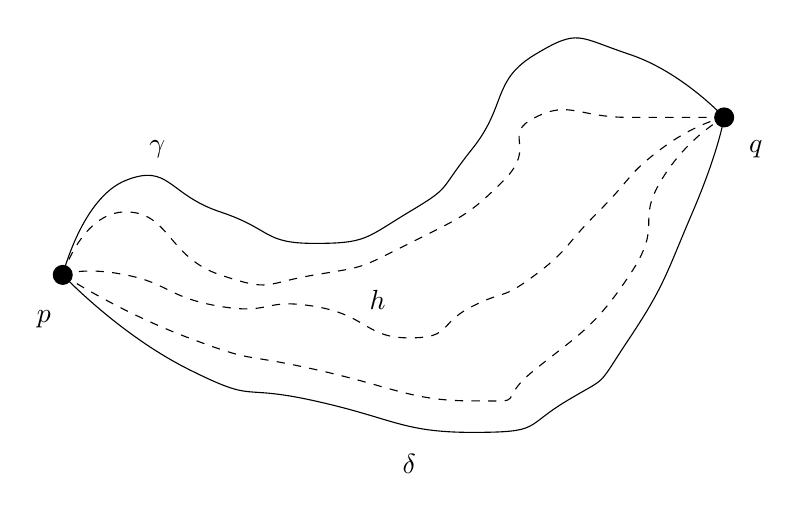
\begin{tikzpicture}[scale=0.8]

\draw  plot[smooth, tension=.999] coordinates {(-3,-0.5) (-2,1) (-0.5,0.5) (1,0) (2.5,0.5) (3.5,1.5) (4.5,3) (6,3) (7.5,2)};

\draw  plot[smooth, tension=.999] coordinates {(-3,-0.5) (-1,-2) (1,-2.5) (3.5,-3) (5,-2.5) (6,-1.5) (7,0.5) (7.5,2)};

\draw[dashed]  plot[smooth, tension=.999] coordinates {(-3,-0.5) (-2,0.5) (-0.5,-0.5) (1,-0.5) (2.5,0) (4,1) (4.5,2) (6,2) (7.5,2)};

\draw[dashed]  plot[smooth, tension=.999] coordinates {(-3,-0.5) (-2,-0.5) (-0.5,-1) (1,-1) (2.5,-1.5) (3.5,-1) (4.5,-0.5) (5.5,0.5) (6.5,1.5) (7.5,2)};

\draw[dashed]  plot[smooth, tension=.999] coordinates {(-3,-0.5) (-1,-1.5) (1,-2) (3.5,-2.5) (4.5,-2) (6,-0.5) (6.5,1) (7.5,2)};

\draw[fill=black]  (-3,-0.5) circle (0.15);
\draw[fill=black]  (7.5,2) circle (0.15);
\node at (-3.3,-1.2) {$p$};
\node at (8,1.5) {$q$};
\node at (-1.5,1.5) {$\gamma$};
\node at (2,-0.9) {$h$};
\node at (2.5,-3.5) {$\delta$};
\end{tikzpicture}
\end{figure}

\begin{proposition}
Let $\gamma \sim \delta :\Leftrightarrow$ ``$\gamma$ and $\delta$ are homotopic''. Then, $\sim$ is an equivalence relation.
\end{proposition}

\begin{mydef}
Let $(M,\mathcal{O})$ be a topological space. Then, for every $p\in M$, we define the \textbf{space of loops} at $p$ by:
$$
\mathcal{L}_p := \{\gamma:[0,1]\to M \mid \gamma \text{ is continuous and } \gamma(0)=\gamma(1)\}.
$$
\end{mydef}

\begin{mydef}
Let $\mathcal{L}_p$ be the space of loops at $p\in M$. We define the \textbf{concatenation} operation $*: \mathcal{L}_p\times\mathcal{L}_p\to\mathcal{L}_p$ by:
$$
(\gamma * \delta) (\l):= \left\{ 
  \begin{aligned}
    \gamma(2\l) & \text{if } 0\leq \l \leq \tfrac{1}{2}\\ 
\delta(2\l-1) & \text{if } \tfrac{1}{2}\leq \l \leq 1 
\end{aligned} 
\right.
$$
\end{mydef}

\begin{mydef}
Let $(M,\mathcal{O})$ be a topological space. The \textbf{fundamental group}\index{fundamental group} $\pi_1(p)$\index{$\pi_1(p)$} of $(M,\mathcal{O})$ at $p\in M$ is the set:
$$
\pi_1(p) := \mathcal{L}_p/\!\sim\ = \{[\gamma] \mid \gamma \in \mathcal{L}_p\},
$$
where $\sim$ is the homotopy equivalence relation, together with the map 
$$ \begin{aligned}
\bullet : & \pi_1(p)\times \pi_1(p) &\to &\pi_1(p)\\
&(\gamma,\delta)&\mapsto & [\gamma]\bullet[\delta]:=[\gamma*\delta] .
\end{aligned} $$
\end{mydef}

\begin{remark}
Recall that a group\index{group} is a pair $(G,\bullet)$ where $G$ is a set and $\bullet : G\times G \to G$ is a map (also called \textbf{binary operation}) such that:
\begin{enumerate}
\item[A)] $\forall \, a,b,c \in G : (a\bullet b)\bullet c = a \bullet (b\bullet c)$;
\item[N)] $\exists \, e \in G : \forall \, g \in G : g \bullet e = e \bullet g = g$;
\item[I)] $\forall \, g \in G : \exists \, g^{-1}\in G: g \bullet g^{-1} = g^{-1} \bullet g = e$.
\end{enumerate}
A group is called \textbf{abelian (or commutative)} if, in addition, satisfies 
\begin{enumerate}
\item[C)] $\forall \, a,b \in G : a\bullet b = b \bullet a$
\end{enumerate}

A \textbf{group isomorphism}\index{isomorphism!of groups} between two groups $(G,\bullet)$ and $(H,\circ)$ is a bijection $\phi: G \to H$ such that:
$$
\forall \, a,b \in G:\phi(a \bullet b) = \phi(a)\circ\phi(b).
$$
If there exists a group isomorphism between $(G,\bullet)$ and $(H,\circ)$, we say that $G$ and $H$ are (group theoretic) isomorphic and we write $G \cong_\mathrm{grp} H$.
\end{remark}

The operation $\bullet$ is associative (since concatenation is associative); the neutral element of the fundamental group $(\pi_1(p),\bullet)$ is (the equivalence class of) the constant curve $\gamma_e$ defined by:
$$ \begin{aligned}
\gamma_e : & [0,1] & \to & M\\
& \l & \mapsto & \gamma_e(0) = p
\end{aligned} $$
Finally, for each $[\gamma]\in\pi_1(p)$, the inverse under $\bullet$ is the element $[-\gamma]$, where $-\gamma$ is defined by:
$$ \begin{aligned}
-\gamma : & [0,1] & \to & M\\
& \l & \mapsto & \gamma(1-\l)
\end{aligned} $$

All the previously discussed topological properties are ``boolean-valued'', i.e.\ a topological space is either Hausdorff or not Hausdorff, either connected or not connected, and so on. The fundamental group is a ``group-valued'' property, i.e.\ the value of the property is not ``either yes or no'', but a group. 

A property of a topological space is called an \textbf{invariant} if any two homeomorphic spaces share the property. A \textbf{classification} of topological spaces would be a list of topological invariants such that any two spaces which share these invariants are homeomorphic. As of now, no such list is known. 

\begin{myex}
The 2-sphere is defined as the set:
$$
S^2:=\{(x,y,z)\in \mathbb{R}^3\mid x^2+y^2+z^2=1\}
$$
equipped with the subset topology inherited from $\mathbb{R}^3$.

\begin{center}
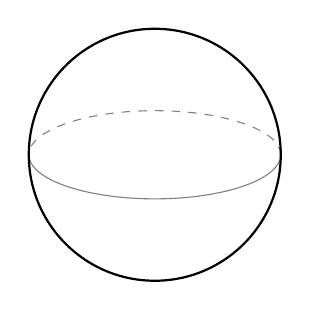
\begin{tikzpicture}[scale=0.8]
  \draw[gray,dashed] (2,0) arc (0:180:2cm and 0.7cm);
  \draw[gray] (2,0) arc (0:-180:2cm and 0.7cm);
  \draw[thick] (0,0) circle[radius=2cm];
\end{tikzpicture}
\end{center}

The sphere has the property that all the loops at any point are homotopic, hence the fundamental group (at every point) of the sphere is the trivial group:
$$
\forall \, p \in S^2 : \pi_1(p) = 1:=\{[\gamma_e]\}.
$$
\end{myex}

\begin{myex}
The cylinder is defined as $C:=\mathbb{R}\times S^1$ equipped with the product topology.

\begin{center}
\begin{tikzpicture}
  \draw[dashed] (-3.75,0) -- (-3,0);
  \draw[dashed] (3,0) -- (3.75,0);
  \draw[dashed] (-3.5,-1.5) -- (3.5,-1.5);
  \draw[dashed] (-3.75,-3) -- (-3,-3);
  \draw[dashed] (3,-3) -- (3.75,-3);
  \draw[thick] (-3,0) -- (3,0);
  \draw[thick] (-3,-3) -- (3,-3);
  \draw[dashed,gray] (0,0) arc (90:-90:0.75cm and 1.5cm);
  \draw[gray] (0,0) arc (90:270:0.75cm and 1.5cm);
\end{tikzpicture}
\end{center}

A loop in $C$ can either go around the cylinder (i.e.\ around its central axis) or not. If it does not, then it can be continuously deformed to a point (the identity loop). If it does, then it cannot be deformed to the identity loop (intuitively because the cylinder is infinitely long) and hence it is a homotopically different loop. The number of times a loop winds around the cylinder is called the \textbf{winding number}\index{winding number}. Loops with different winding numbers are not homotopic.

Moreover, loops with different \textbf{orientations} are also not homotopic and hence we have:
$$
\forall \, p \in C : (\pi_1(p),\bullet) \cong_\mathrm{grp}(\mathbb{Z},+).
$$
\end{myex}

\begin{myex}
The 2-torus is defined as the set $T^2:=S^1\times S^1$ equipped with the product topology.
\begin{center}
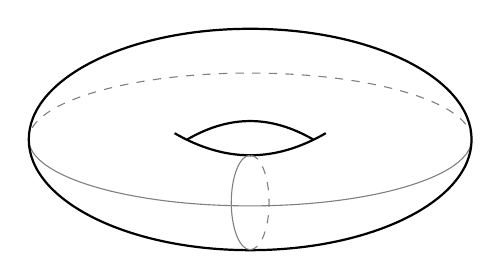
\begin{tikzpicture}[scale=0.8]
  \draw[thick] (-1,0) to[bend left] (1,0);
  \draw[thick] (-1.2,.1) to[bend right] (1.2,.1);
  \draw[gray] (100pt,0) arc (0:-180:100pt and 30pt);
  \draw[gray,dashed] (100pt,0) arc (0:180:100pt and 30pt);
  \draw[thick] (0,0) ellipse (100pt and 50pt);
  \draw[gray,dashed]  (0,-1.75) arc (-90:90:0.3 and 0.75);
  \draw[gray] (0,-1.75) arc (-90:-270:0.3 and 0.75);
  \end{tikzpicture}
\end{center}
A loop in $T^2$ can intuitively wind around the cylinder-like part of the torus as well as around the hole of the torus. That is, there are two independent winding numbers and hence:
$$
\forall \, p \in T^2 : \pi_1(p) \cong_\mathrm{grp}\mathbb{Z}\times \mathbb{Z},
$$
where $\mathbb{Z}\times \mathbb{Z}$ is understood as a group under pairwise addition.
\end{myex}
%}}}

\chapter{Topological manifolds}%{{{
Roughly, a topological manifold is a topological space that locally looks like $\mathbb{R}^d$.
\begin{mydef}
  A paracompact Housdorff topological space $(M, \mathcal{O})$ is called a d-dimensional (topological) \textbf{manifold} if for every $p\in M: \exists p \in U \in \mathcal{O}$ and a homeomorphism $x:U \rightarrow x(U) \subseteq \mathbb{R}^d$
\end{mydef}
\begin{mydef}
  Let $(M,\mathcal{O})$ be a d-dimensional topological manifold and $N \subset M$. Then, $(N,\mathcal{O}\mid_N)$ is a \textbf{submanifold} of $(M,\mathcal{O})$ if it is a manifold in its own right.
\end{mydef}
\begin{mydef}
  Let $(M,\mathcal{O}_M)$ and $(N,\mathcal{O}_N)$ be a topological manifolds. Then, $(M\times N, \mathcal{O}_M \times \mathcal{O}_N)$ is a manifold of dimension $dim(M) + dim(N)$ called the \textbf{product manifold}. ``We attach a copy of the second manifold to each point of the first''.
\end{mydef}
\section{Viewing manifolds from atlases}
\begin{mydef}
  Let $(M,\mathcal{O})$ be a d-dimensional topological manifold. Then, a pair $(U,x)$ where $U\in \mathcal{O}$ and $x : U \rightarrow x(U) \subseteq \mathbb{R}^d$ is a \textbf{chart} of the manifold. The component functions of $x$,
$$ 
\begin{aligned}
  x_i :& U   & \to     & \mathbb{R}\\
       & p   & \mapsto & proj_i(x(p))
\end{aligned} 
$$
are called the \textbf{coordinates} of the point $p$ with respect to the chart $(U,x)$.
\end{mydef}
\begin{remark}
  There exists a set of charts $\mathcal{A}$ such that $\bigcup U_i = M,\ (U_i, x_i) \in \mathcal{A}$. $\mathcal{A}$ is called \textbf{atlas}.
\end{remark}

\begin{mydef}
  Two charts $(U,x)$ and $(V,y)$ are called $\boldsymbol{\mathcal{C}^0}$\textbf{-compatible} if either
  \begin{enumerate}
    \item $U\cap V = \emptyset$
    \item $U\cap V \neq \emptyset : y \circ x^{-1}$ is continuous.
  \end{enumerate}
% Note that $y\circ x^{-1}$ is a map from a subset of $\R^d$ to a subset of $\R^d$.
% \bse
% \begin{tikzcd}
% & U\cap V \se M \ar[ldd,"x"'] \ar[rdd,"y"]&\\
% &&&\\
% x(U\cap V) \se \R^d \ar[rr,"y\circ x^{-1}"']& & y(U\cap V)\se \R^d
% \end{tikzcd}
% \ese
\end{mydef}

\begin{remark}
  The map $y \circ x^{-1}: \mathbb{R}^d \to \mathbb{R}^d$ is also called the \textbf{coordinate change chart}.
\end{remark}

\begin{remark}
  Continuity can be described at a topological level, but not differentiability. For that we have to use the chart-transition maps.
\end{remark}

%}}}

\chapter{Algebraic structures}%{{{
\section{Group}
\begin{mydef}
  A \emph{group} $(G,\bullet)$ is a set $G$ equipped with a map
  \begin{align*}
    \bullet\ :\ &G \times G \rightarrow G\\
                &(g_1, g_2) \mapsto g_1 \bullet g_2
  \end{align*}
  that satisfies $ANI$ (Associative, Neutral element and Inverse element). If the map is commutative $(CANI)$, the group is said to be commutative or abelian.
\end{mydef}
\section{Ring}
\begin{mydef}
  A \emph{ring} $(R, +, \cdot )$ is a set $R$ equipped with two maps
  \begin{align*}
    +      &:\ R \times R \rightarrow R\\
    \cdot\ &:\ R \times R \rightarrow R\\
  \end{align*}
  that satisfies $C^{+}A^{+}N^{+}I^{+}$ for $R$ and $A^{\cdot}N^{\cdot}D^{\cdot}_{+}$  for $R\setminus \{0\}$. Where $D^{\cdot}_+$ means $\cdot$ is distributive wrt $+$.
\end{mydef}

\section{Field}
\begin{mydef}
  A \emph{field} (algebraic field) $(K, +, \cdot )$ is a set $K$ equipped with two maps
  \begin{align*}
    +      &:\ K \times K \rightarrow K\\
    \cdot\ &:\ K \times K \rightarrow K\\
  \end{align*}
  that satisfies $C^{+}A^{+}N^{+}I^{+}$ for $K$ and $C^{\cdot}A^{\cdot}N^{\cdot}I^{\cdot}D^{\cdot}_{+}$ for $K\setminus \{0\}$ 
\end{mydef}
\section{Module}
\begin{mydef}
  A \emph{R-module} $(M, \oplus, \odot )$ over a ring $(R, +, \cdot)$ is a set $M$ equipped with the maps
  \begin{align*}
    \oplus      :\ &M \times M \rightarrow M\\
    \odot       :\ &R \times M \rightarrow M\\
                &\ r \odot m \mapsto r\cdot m\\
  \end{align*}
  that satisfies $C^{\oplus}A^{\oplus}N^{\oplus}I^{\oplus}$ and $AD^{\odot}_+D^\odot_{\oplus}U^{\odot}$. $U$ stands for unitary.
\end{mydef}
\section{Vector space}
\begin{mydef}
  A \emph{K-vector space} $(V, \oplus, \odot )$ over a field $(K,+,\cdot)$ is a set $V$ equipped with the maps
  \begin{align*}
    \oplus  :\ &V \times V \rightarrow V\\
    \odot   :\ &K \times V \rightarrow V\\
            &\ k \odot v \mapsto k\cdot v\\
  \end{align*}
  that satisfies $C^{\oplus}A^{\oplus}N^{\oplus}I^{\oplus}$ and $AD^{\odot}_+D^\odot_{\oplus}U^{\odot}$. A module is a vector space structure over a ring, i.e. non-commutative $\cdot$.
\end{mydef}
\begin{mydef}
  $U \subset V$ is a vector subspace if $\forall u, u_1, u_2 \in U$  
  \begin{align*}
    &u_1 \oplus u_2 \in U\\
    &\lambda \odot u \in U
  \end{align*}
\end{mydef}

%}}}

\chapter{Linear maps}%{{{
  \section{Linear Map}
  \begin{mydef}
    Let $(V,\oplus,\odot),(W,\boxplus,\boxdot)$ be vector spaces over the same field $(K, +,\cdot)$. A map $f : V \rightarrow W$ is linear if
    \begin{align*}
      & \forall v_1, v_2 \in V && f(v_1 \oplus v_2) = f(v_1) \boxplus f(v_2)\\
      & \forall \lambda \in K,\ v\in V && f(\lambda \odot V) = \lambda \boxdot f(v)
    \end{align*}
  \end{mydef}
  \begin{mydef}
    Linear maps are the structure-preserving maps of vector spaces, i.e. the vector-space homomorphisms. The set containing all linear maps is defined as:
    $$
    Hom(V,W) := \{ f : V \tilde{\longrightarrow} W\}
    $$
  \end{mydef}
  \begin{mydef}
    $(Hom(V,W), +_H, \cdot_H)$ can be made into a vector space by inducing the operators from $W$.
  \end{mydef}
  \begin{mydef}
    A linear map is called endomorphism if $V=W$
  \end{mydef}
  \begin{mydef}
    A bijective linear map is called a vector space isomorphism
    $$
    V \cong_{vec} W \Leftrightarrow \exists f : V \tilde{\longrightarrow} W \mid f \text{ bijective}
    $$
  \end{mydef}
  \subsection*{Terminology}
  \begin{mydef}
    Endomorphisms $\equiv End(V) := Hom(V,V)$
  \end{mydef}
  \begin{mydef}
    Automorphisms $\equiv Aut(V) := End(V)$ invertible.
  \end{mydef}
  \begin{mydef}
    Dual vector space $\equiv V^* := Hom(V,K)$. Heavily used. $V^*$ is the set of linear functions.
  \end{mydef}

  \section{Linear independence. Basis}
  \begin{mydef} 
    Let $V$ be a vector space. Then, $S = \lbrace{s_1, \ldots, s_n \rbrace}\subseteq V$ is \textbf{linearly independent} if the linear combination of the vectors $s_i$ is only degenerate for the degenerate linear combination. Mathematically,
    $$
    \sum_{i=1}^n \lambda_i s_i = 0, \lambda_i \in K \Rightarrow \lambda_i = 0, \forall i = 1, \ldots, n
    $$
  \end{mydef} 
  \begin{mydef}
    $S\subset V$ is a \textbf{generating system} iff
    $$
    \forall v \in V\ \exists \lbrace \lambda_1, \ldots, \lambda_n \rbrace : \sum_{i=1}^n \lambda_i s_i = v
    $$
    which is denoted by $V = \langle S \rangle$
  \end{mydef}
  \begin{mydef}
    A linearly independent generating system is called a \textbf{basis}.
  \end{mydef} 
  \begin{remark}
  One can choose arbitrary basis for $V$ and $V^*$. However, it's more economical to derive the basis on $V^*$ based on the choice of basis in $V$.
  $$
  \epsilon^a(e_b) = \delta^a_b
  $$
  This uniquely determines the choice of $\epsilon^1, \ldots, \epsilon^n$ for a given choice of $e_1, \ldots, e_n$. This is called a \textbf{dual basis} of $V$.
  \end{remark}
  \begin{myex}
    Consider the 3rd degree polynomials. Then, a basis $\{e_0, e_1, e_2, e_3\} = \{1, x, x^2, x^3\}$ can be defined and a dual basis can be defined as  
    $$
    \{\epsilon^0,\epsilon^1,\epsilon^2,\epsilon^3\} : \epsilon^a = \frac{1}{a!}\partial^a (\cdot) \mid_{x=0} = \delta^a_b
    $$
  \end{myex}
  \subsection{Change of basis}

  \section{Kernel and image of a linear map}
  \begin{mydef}
    Let $f:V\rightarrow W$ be a linear map. Then, its \textbf{kernel} is defined as:
    $$
      Ker(f) := x \in V : f(x) = 0
    $$
    The kernel $Ker(f)$ and image $Im(f)$ are vector subspaces of $V$ and $W$ respectively, with
    $$
    dim(Ker(f)) + dim(Im(f)) = dim(V)
    $$
  \end{mydef} 

%}}}

\chapter{Multilinear maps: Tensors}%{{{
\begin{mydef}
  Let $(V,+,\cdot)$ be a K-vector space. A $(p,q)-$tensor $T$ over $V$ is a multilinear map
  $$
  T: \underbrace{V^* \times \cdots \times V^*}_{\text{p copies}} \times \underbrace{V \times \cdots \times V}_{\text{q copies}} \tilde{\longrightarrow} K
  $$
\end{mydef}
\begin{myex}
  $$
  \begin{aligned}
  &\varphi \in V^* \Leftrightarrow \varphi : V \tilde{\longrightarrow} K \Leftrightarrow \varphi \text{ is a $(0,1)-$tensor.}\\
  & v \in V \Leftrightarrow v \in \left( V^*\right)^* \Leftrightarrow v: V^* \tilde{\longrightarrow} K \Leftrightarrow v \text{ is a $(1,0)-$tensor.}
  \end{aligned}
  $$
  In addition, linear maps are $(1,1)-$tensor. An inner product on a vector space is a $(0,2)-$tensor. The ``inverse'' or dual inner product is a $(2,0)-$tensor.
\end{myex}

\section{Components of tensors}
\begin{mydef}
  Let T be an $(p,q)-$tensor over a finite-dimensional vector space V. Then, define the $(p+q)^{dim(V)}$ real numbers.
  $$
  T^{i_1,\ldots, i_p}{}_{j_1, \ldots, j_q} := T(\epsilon^{i_1}, \ldots, \epsilon^{i_p}, e^{j_1}, \ldots, e^{j_q}) \in K
  $$
\end{mydef}
\subsection{Reconstruction of T from its components}
\begin{myex}
  T is a $(1,1)-$tensor. Then,
  $$
  T^i{}_j := T(\epsilon^i, e_j)
  $$
  thus,
  $$
  T(\varphi,v) = T(\sum_{i=1}^{dimV}\varphi_i \epsilon^i, \sum_{j=1}^{dimV}v^j e_j) = 
  \sum_{i=1}^{dimV}\sum_{j=1}^{dimV}\varphi_i v^j T(\epsilon^i,  e_j) =: \varphi_i v^j T^i{}_j 
  $$
  where the last term is written in Einstein summation convention, where up-down matching indices are summed over.
\end{myex}

%}}}

\chapter{Differentiable manifolds}%{{{
\section{Adding structure by refining the (maximal) topological atlas}
\begin{mydef}
  Let $(M, \mathcal{O})$ be a manifold. An atlas $\mathcal{A}$ is called a $\clubsuit-$\textbf{atlas} if any two charts $(U,x), (V,y) \in \mathcal{A}$ are $\clubsuit-$compatible. In other words, either:
  \begin{itemize}
    \item $U\cap V = \emptyset$
    \item $U\cap V \neq \emptyset \Rightarrow y\circ x^{-1}$ must be $\clubsuit$ as a $\mathbb{R}^d \to \mathbb{R}^d$ map.
  \end{itemize}
  Where $\clubsuit$ can be:
  \begin{itemize}
    \item $C^0$
    \item $C^k$: The transition maps are k-times continuously differentiable (traditional def.)
    \item $C^\infty$: Smooth.
    \item $C^\omega$: Real analytic (Can be Taylor expanded).
    \item Complex: Transition functions satisfy the Cauchy-Riemman equations.
  \end{itemize}
\end{mydef}
\begin{theorem}
  Any maximal $C^{k\geq 1}-$atlas contains a $C^\infty -$atlas. Two maximal $C^k-$atlasses that contain the same $C^\infty-$atlas are identical. This implies that you do not need to distinguish between $C^{k\geq 1}$ and $C^\infty$ in the previous sense.
\end{theorem}

\begin{mydef}
  A $C^k-$manifold is a triple $(M, \mathcal{O}, \mathcal{A})$ where $(M,\mathcal{O})$ is a topological manifold and $\mathcal{A}$ is a $C^k-$atlas.
\end{mydef}

\begin{mydef}
  Let $\phi : M \to N$ be a map, where $(M, \mathcal{O}_M, \mathcal{A}_M)$ and $(N, \mathcal{O}_N, \mathcal{A}_N)$ are $C^k-$manifolds. Then, $\phi$ is called \textbf{differentiable} at a point $p \in M$ if for some $(U,x)\in \mathcal{A}_M$ with $p\in U$ and some chart $(V,y) \in \mathcal{A}_N$ with $\phi(p)\in V$ the map $y\circ \phi \circ x^{-1}$ is $C^k$ as a map from $\mathbb{R}^{dim(M)} \to \mathbb{R}^{dim(N)}$.
\end{mydef}
\begin{mydef}
  If $\phi M \to N$ is bijective and both $\phi$ and $\phi^{-1}$ are $C^\infty$, then $\phi$ is called \textbf{diffeomorphism}. They are the structure preserving maps over differentiable manifolds. 
\end{mydef}
\begin{mydef}
  $(M, \mathcal{O}_M, \mathcal{A}_M)$ and $(N, \mathcal{O}_N, \mathcal{A}_N)$ are called diffeomorphic if there exist a diffeomorphism between them.
  $$
  M \cong_{diff} N \equiv  (M, \mathcal{O}_M, \mathcal{A}_M) \cong_{diff}(N, \mathcal{O}_N, \mathcal{A}_N)
  $$
\end{mydef}
\begin{remark}
  It is custom to consider diffeomorphic smooth manifolds to be the same.
\end{remark}
\begin{remark}
  The key feature of the differentiable manifolds is that exists a \textbf{tangent} (vector) \textbf{space} at each point of the manifold.
\end{remark}

\section{Tangent spaces to a manifold}
\begin{mydef}
  Let M be a smooth manifold. Then, we can construct the vector space over $\mathbb{R}: (C^\infty(M), +, \cdot)$ where the operators are inherited from $\mathbb{R}$ and $C^\infty(M)$ is the set of all smooth functions on the manifold $f:M\to \mathbb{R}$.
\end{mydef}
\begin{mydef}
  Let $\gamma : \mathbb{R} \to M$ be a smooth curve through a point $p\in M$. Without loss of generality (w.l.o.g.), we may arrange for $p = \gamma(0)$. \textbf{ The directional derivative operator} at $p$ along the curve $\gamma$ is a linear map:
  $$
  \begin{aligned}
    X_{\gamma, p} : C^\infty(M) &\to \mathbb{R}\\
    \quad f    &\mapsto (\underbrace{f \circ \gamma}_{\mathbb{R}\to \mathbb{R}})'(0)
  \end{aligned}
  $$
  In differential geometry, $X_{\gamma, p}$ is usually called the \textbf{tangent vector} to the curve $\gamma$ at the point $p\in M$. It is also called the velocity of $\gamma$ at $p$.
\end{mydef}

\begin{mydef}
  The \textbf{tangent vector space} is the set
  $$
  T_pM:=\left\{ X_{\gamma, p}\ \forall\ \gamma \text{ smooth curves through } p\right\}
  $$
  equipped with:
  $$
  \begin{aligned}
    \oplus &: T_pM \times T_pM \to T_pM\\
    \odot  &: \mathbb{R} \times T_pM \to T_pM
  \end{aligned}
  $$
  We can directly inherit the operators from $\mathbb{R}$.
  $$
  \begin{aligned}
    (X_{\gamma,p} \oplus X_{\delta,p})(f) &:= X_{\gamma, p}(f) + X_{\delta, p}(f)\\
    (\lambda \odot X_{\gamma,p})(f) &:= \lambda \cdot X_{\gamma, p}(f)
  \end{aligned}
  $$
\end{mydef}

%}}}

\chapter{Lie groups and their Lie algebras}%{{{

%}}}

\chapter{Construction of \emph{SE(3)}}%{{{

%}}}

\onlyinsubfile{
\bibliography{bibliography} %Same name as .bib
\addcontentsline{toc}{chapter}{Bibliography}
\bibliographystyle{abbrv}
}
\end{document}
